\section{Introduction}\label{sec-nbcp-introduction}
\begingroup
\setlength{\intextsep}{9pt plus 1pt minus 1pt}

A spin supersolid combines longitudinal magnetic density order with
transverse phase coherence. In U(1)-symmetric easy-axis triangular
antiferromagnets, the Y and V supersolids flank the one-third up--up--down
magnetization plateau. Recent experiments probe this coexistence in
several cobalt compounds (Table~\ref{tab-nbcp-materials}).

\begin{table}[H]
\centering
\small
\renewcommand{\arraystretch}{1.12}
\begin{tabular}{@{}clc@{}}
\toprule
\textbf{Material} & \textbf{Recent evidence} & \textbf{Ref.} \\
\midrule
\multirow[c]{2}{*}{\(\mathrm{Na_2BaCo(PO_4)_2}\)} &
Magnetocaloric and diffraction signatures (2024) & \cite{xiang2024} \\
&
NMR supports Y/V order and gapless excitations (2025) & \cite{nmr2025} \\
\addlinespace[3pt]
\multirow[c]{2}{*}{\(\mathrm{K_2Co(SeO_3)_2}\)} &
Neutron signatures of supersolidity (2026) & \cite{kcso2026} \\
& Resolved transverse order (July 2026 preprint) & \cite{zhu2026} \\
\addlinespace[3pt]
\(\mathrm{Rb_2Co(SeO_3)_2}\) &
NMR/thermodynamics consistent with supersolidity (2026) & \cite{rb2026} \\
\bottomrule
\end{tabular}
\caption{Recent spin-supersolid evidence in cobalt compounds.}
\label{tab-nbcp-materials}
\end{table}

We focus on \(\mathrm{Na_2BaCo(PO_4)_2}\) (NBCP), an effective
spin-\(1/2\) triangular-layer magnet described by easy-axis
exchange~\cite{gao2022}. Crystal fields and atomic spin-orbit coupling
(SOC) form the low-energy doublet; residual bond-dependent exchange can
break continuous spin-rotation symmetry.

\begin{figure}[H]
\centering
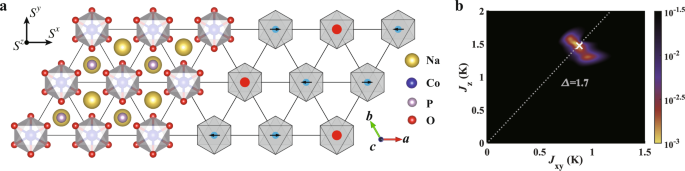
\includegraphics[width=0.55\linewidth,trim=0 0 242bp 0,clip]{sources/figures/gao-2022-figure-1.png}
\caption{NBCP layer and proposed spin texture: circles and arrows denote
longitudinal and transverse components. Cropped from Ref.~\cite{gao2022},
Fig.~1(a); \href{https://creativecommons.org/licenses/by/4.0/}{CC BY 4.0}.}
\label{fig-nbcp-crystal-structure}
\end{figure}

Does Y/V supersolidity survive this symmetry breaking?
Park et al.~\cite{park2026} predict SOC-induced zero-temperature gaps
but thermal stabilization of certain supersolid states. We examine the
microscopic basis of this scenario through:
\begin{itemize}[itemsep=2pt,topsep=3pt]
\item \textbf{Magnetic phases:} the symmetry-allowed Hamiltonian,
classical orders, zero-point corrections and competing states,
including the proposed skyrmion lattice.
\item \textbf{Y/V dynamics:} quantum pinning, pseudo-Goldstone gaps
and phase stiffness, and their connection to clock-model and
renormalization-group criteria.
\end{itemize}
Nonlinear Y gradients and density walls test part of this description.
Vortex and finite-temperature matching remain necessary to establish
microscopic thermal supersolidity.

\endgroup
